\section{The context}

\section{The web}
\subsection{Basic structure}
\subsection{The web browser}
\subsection{JavaScript}

\section{WebAssembly}
\subsection{Description and motivations}
\subsection{Problems with WebAssembly}
\subsection{WebAssembly as a fault isolation tool}
\subsection{WASI - WebAssembly System Interface}

\section{Linux Security Modules}

The \textit{Linux Security Module} (LSM) \cite{lsm-2002} \cite{kernel-lsm}
is a lightweight, general purpose, access control framework for the Linux Kernel.
It provides a mechanism for various security checks to be hooked by kernel extensions.
These extensions are not loadable kernel modules, but they can either be choosen at
compile-time via specific flags, such as \texttt{CONFIG\_DEFAULT\_SECURITY}, or overridden at boot-time.

The LSM is used primarily by \textit{Mandatory Access Control} (MAC) extensions to
provide a security policy. However, other extensions can be built with the LSM framework
in order to implement specific changes when they cannot be obtained with the functionality Linux itself.

Some projects that use LSM include:
\begin{itemize}
  \item \textit{SELinux} \cite{selinux}, i.e.\ \textit{Security Enhanced Linux}, that provides a mechanism for supporting advanced and fine-grained access control policies, as well as MAC;
  \item \textit{Smack} \cite{smack}, a kernel based implementation of MAC with simplicity as one of its primary goals;
  \item \textit{AppArmor} \cite{apparmor}, a MAC style security extension that implements a task centered policy.
\end{itemize}

\begin{figure}[h]
  \centering
  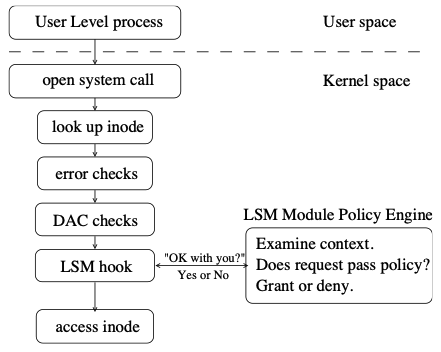
\includegraphics[width=0.5\linewidth]{lsm-hook-architecture.png}
  \caption{LSM Hook Architecture, from \cite{kernel-lsm}}
  \label{fig:lsm-hook-architecture}
\end{figure}

\subsection{Landlock}
\textit{Landlock} \cite{landlock-kernel} \cite{landlock-user-space} is a security feature available since Linux 5.13
that uses the LSM framework in order to provide scoped access control,
so that any process, even when unprivileged, can securely restrict itself.
This can help mitigate the security impact of bugs or unexpected/malicious behaviour
in user space applications.

Landlock employes the concept of \textit{rule}, which describes an action
on an object. An object is (currently) a file hierarchy, and actions are
defined with access rights, such as executing, reading or writing files, making
symbolic links and so on.
A set of rules is called a \textit{ruleset}, and it can restrict both the thread
using it and its future children, created either by spawning a new thread, as well
as using the \textit{fork} system call.

Notably, Landlock does not permits the definition of exeptions.
For example, suppose we have a directory \texttt{dir1}, which contains two files
\texttt{file1} and \texttt{file2}. We can define a ruleset that allows
reading and writing files for \texttt{dir1}.
However, if we then define another ruleset comprising only of read operations
for \texttt{file1}, the permissions specified for \texttt{dir1} are still
valid, so when a process restricts itself it is still able to write to \texttt{file1}.

In case of multiple consecutive self-restrictions, the result is the intersection
of all rulesets - if a process first restricts itself allowing all read and writing operations,
and then restricts itself again with only reading permissions, the result is equivalent
to a single restriction made with a ruleset that permits only reading operations.

\subsection{BPF}